\documentclass[11pt,a4paper]{article}

\usepackage[utf8]{inputenc}
\usepackage[english]{babel}
\usepackage[T1]{fontenc}

\usepackage{amsmath,amssymb,amsfonts}
\usepackage{hyperref}
\usepackage{graphicx}

\title{Computational Geometry - Range Searching}
\author{Philip Munksgaard \\ Sebastian Paaske Tørholm \\ Ejnar Håkonsen}

\begin{document}
\maketitle

\section{Exercise 5.1}

We use the first rule of the master theorem~\cite{Cormen theorem 4.1}
to solve the recurrence. Since $a=2, b=4, f(n)=2$, we get that $\log_b a
= \frac{1}{2}$ and thus we get $Q(n) = \Theta(\sqrt{n})$.

Given that $Q(n) = \Theta(\sqrt{n})$, we also have $Q(n) = \Omega(\sqrt{n})$
as desired.

\begin{figure}[h!]
    \centering
    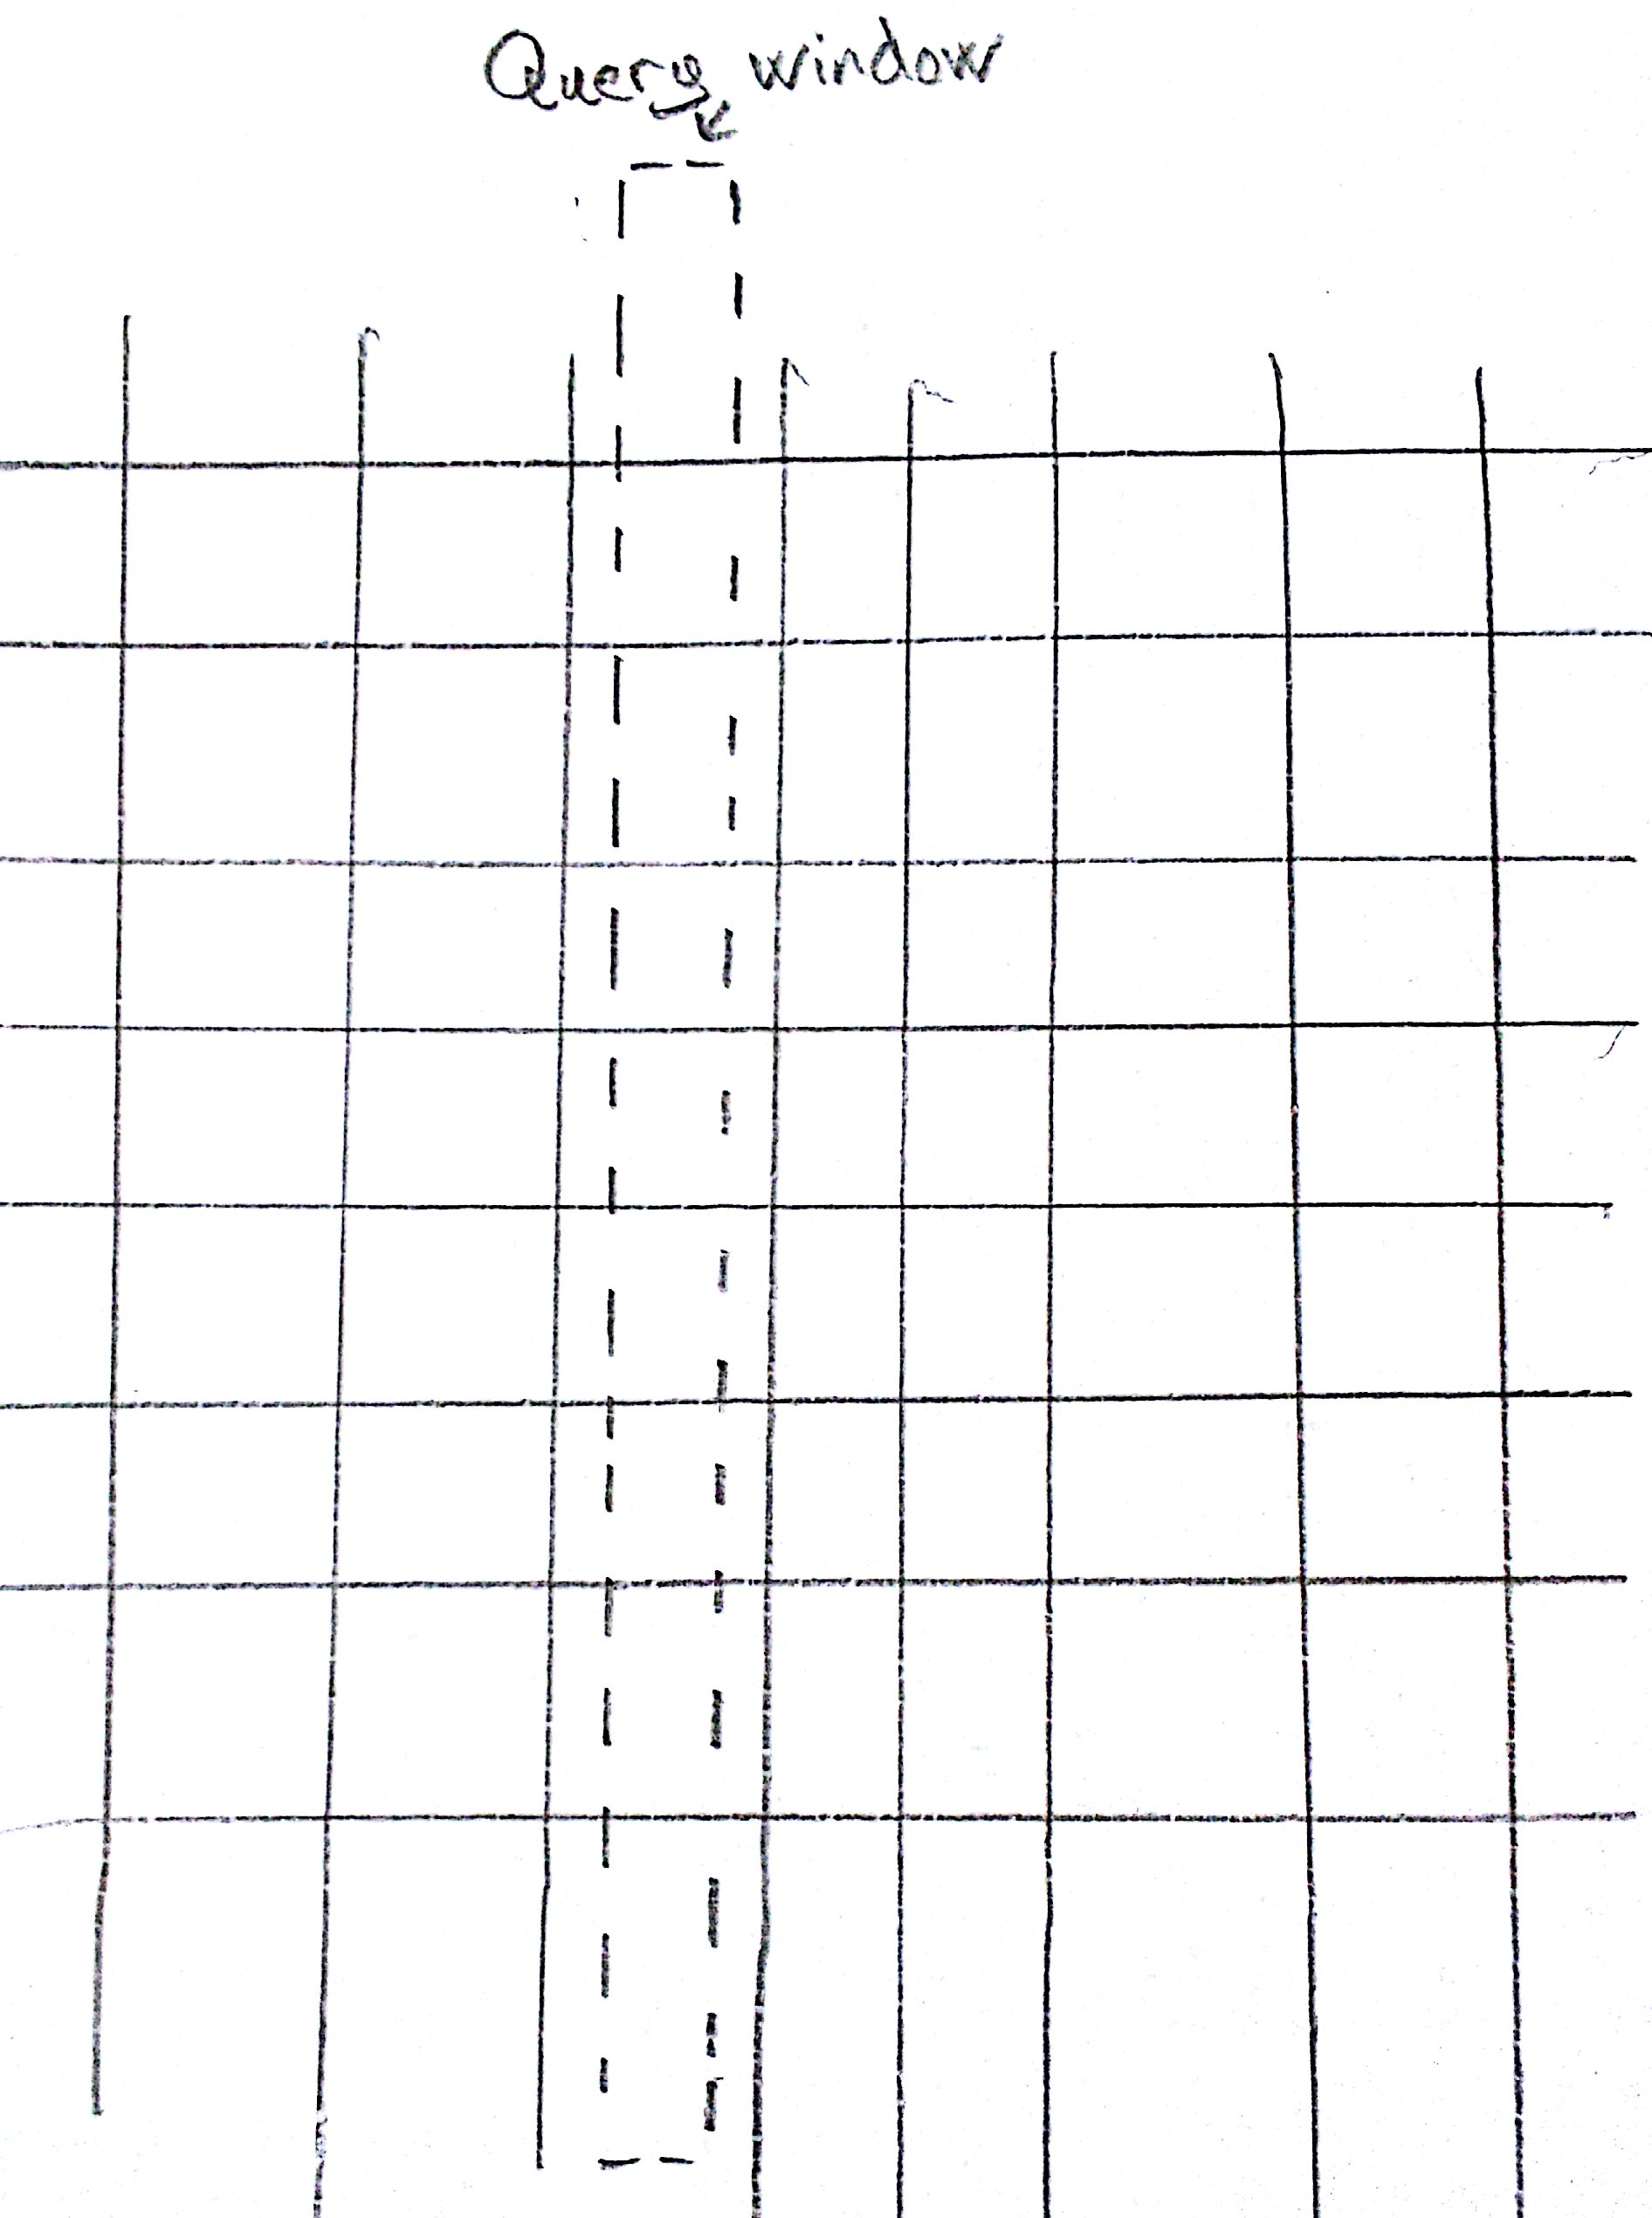
\includegraphics[width=.6\textwidth]{tegning-ex51.jpg}
    \caption{Construction for the worst case in exercise 5.1}
    \label{tegning-ex51}
\end{figure}

We can see an example of such a worst case by constructing a $m \times m$ grid
of evenly spaced points. It's easy to convince oneself that the splitting of
the plane done by the $kd$-tree will contain the lines of the grid.
\footnote{Minor tweaking of $x$ and $y$ coordinates is necessary to make
them distinct, but the idea should hold nonetheless.}

Let us then consider a query window starting above the grid, and ending below it,
placed such that it doesn't contain any points. (See \autoref{tegning-ex51})
This window will intersect at least $m$ lines, and overlap with at least $m+1$
regions. If we let $n = m^2$, we get $\sqrt{n}+1$ regions we must check, and
as such is an example of the worst case.

\section{Exercise 5.10}

\subsection{Exercise 5.10a}

We can easily modify the 1-dimensional range tree to accommodate range
counting queries by letting each node store an integer that indicates
how many leafs that nodes' tree contains. Then, querying becomes a
simple matter of finding the nodes which we'd normally call
\verb+ReportSubtree+ on (reporting all their children) and instead
simply report how many leafs are in that sub-tree.

Proving that this modified 1-dimensional range tree lets us query for
range counts in $O(\log n)$ time, is a simple matter of recalling that
the query time for normal range queries in a 1-dimensional range tree
is $O(\log n + k)$, where the $k$ is the time spent in calls to
\verb+ReportSubtree+. In our range counting queries, we have
substituted the calls to \verb+ReportSubtree+ for a constant time
operation (reporting the number stored in the node), and it thus
follows that the query time must be $O(\log n + 1) = O(\log n)$.

\end{document}
